\documentclass{beamer}
\usetheme{metropolis}
\usepackage{graphicx}
\title{Calculus-Based Physics-1: Mechanics (PHYS150-01): Week 1}
\date{September 6th - September 8th, 2017}
\author{Jordan Hanson}
\institute{Whittier College Department of Physics and Astronomy}

\begin{document}
\maketitle

\begin{frame}{Course Introduction}
\begin{enumerate}
\item Professor Jordan Hanson
\item Contact: 918particle@gmail.com, SLC 200
\item Syllabus: whittier.edu
\item Office hours: Mondays, Tuesdays at 15:00
\item Course pre-requisites: Calculus 1 (concurrently)
\item Text: University Physics Volume 1 (openstax.org)
\item Homework: ExpertTA (theexpertta.com)
\end{enumerate}
\end{frame}

\begin{frame}{Week 1 Summary}
\textit{Physics} - $\phi\upsilon\sigma\iota\kappa\acute{\eta}$ - "phusik\'e": \textit{knowledge of nature} \\
from $\phi\acute{\upsilon}\sigma\iota\varsigma$ - "ph\'usis": \textit{nature}
\begin{enumerate}
\item Methods of approximation
\begin{itemize}
\item \alert{Estimating} the correct order of magnitude
\item \alert{Function} approximation
\item \alert{Unit analysis}
\end{itemize}
\item Coordinate systems and vectors
\begin{itemize}
\item \alert{Cartesian} (rectangular) coordinates
\item \alert{Vector} addition and subtraction
\item \alert{Time} and relativity
\end{itemize}
\item Some concepts from single-variable calculus
\begin{itemize}
\item Limits
\item Differentiation
\item Integration
\end{itemize}
\end{enumerate}
\end{frame}

\section{Methods of approximation}

\begin{frame}{Methods of approximation - Estimation (Chapter 1.5)}
In science and engineering, \alert{estimation} is to obtain a quantity in the absence of precision, informed by rational constraints.
\begin{enumerate}
\item Define relevant \alert{scales}
\begin{itemize}
\item 1 \textit{AU} for the solar system (distance from Sun to Earth)
\item 1 \textit{angstrom} ($10^{-10}$ meters) for cell membranes
\end{itemize}
\item Obtain \alert{complex quantities} from simple ones
\begin{itemize}
\item Obtain \textit{areas} and \textit{volumes} from \textit{lengths}
\item Obtain \textit{rates} from \textit{numerators} and \textit{denominators}
\end{itemize}
\item Constrain the unknown with \alert{upper} and \alert{lower} limits
\begin{itemize}
\item The solar system is \textit{less than one light-year across}
\item An insect is \textit{at least one millimeter} long
\end{itemize}
\end{enumerate}
\end{frame}

\begin{frame}{Methods of approximation - Estimation (Chapter 1.5)}
\small
\begin{minipage}[b]{0.45\linewidth}
Estimate the mass of ants in an ant colony.  Assume that the colony is a species known to have $10^5$ ants (roughly) per colony.
\begin{itemize}
\item A: 0.01 kg
\item B: 0.1 kg
\item C: 1 kg
\item D: 10 kg
\end{itemize}
\end{minipage}
\hspace{0.5cm}
\begin{minipage}[b]{0.45\linewidth}
An adult blue whale is about 30 meters long.  What is the mass of a blue whale calf? (1 tonne = 1000 kg).
\vspace{0.55cm}
\begin{itemize}
\item A: 100 kg
\item B: 0.5 tonnes
\item C: 5 tonnes
\item D: 20 tonnes
\end{itemize}
\end{minipage}
\end{frame}

\begin{frame}{Methods of approximation - Estimation (Chapter 1.5)}
\small
\begin{minipage}[b]{0.45\linewidth}
How long does it take an airliner to fly across the Atlantic ocean?  Assume the velocity is 500 mph, and the radius of the Earth is 7000 km.
\vspace{0.6cm}
\begin{itemize}
\item A: 10 hours
\item B: 15 hours
\item C: 2 hours
\item D: 4 hours
\end{itemize}
\end{minipage}
\hspace{0.5cm}
\begin{minipage}[b]{0.45\linewidth}
A flock of birds takes one minute to pass overhead, and it is about 100 meters wide, with most birds flying at roughly the same altitude.  How many birds are in the flock?
\vspace{0.1cm}
\begin{itemize}
\item A: 100 birds
\item B: 1,000 birds
\item C: 10,000 birds
\item D: 100,000 birds
\end{itemize}
\end{minipage}
\end{frame}

\begin{frame}{Methods of approximation - Function approximation}
In science and engineering, \alert{function approximation} or \alert{expanding a function} is a technique in which a simple function is used obtain the value of a more complicated function near a point where they are approximately equal. 
\begin{enumerate}
\item Memorizing \alert{special cases}
\begin{itemize}
\item $\sin(x) \approx x$, when $|x| < 1$
\item $\tan(x) \approx x$, when $|x| < 1$
\item $(1+x)^{1/2} \approx 1+ \frac{1}{2}x$, when $|x| < 1$
\item $\exp(x) \approx 1 + x$, when $|x| < 1$
\end{itemize}
\item Utilizing the \textbf{Taylor Series} (more on this later)
\begin{itemize}
\item $f(x) \approx f(a) + \frac{f'(a)}{1!}(x-a) + \frac{f''(a)}{2!}(x-a)^2 + \frac{f'''(a)}{3!}(x-a)^3 + ...$
\end{itemize}
\end{enumerate}
\end{frame}

\begin{frame}{Methods of approximation - Function approximation}
\begin{figure}
\centering
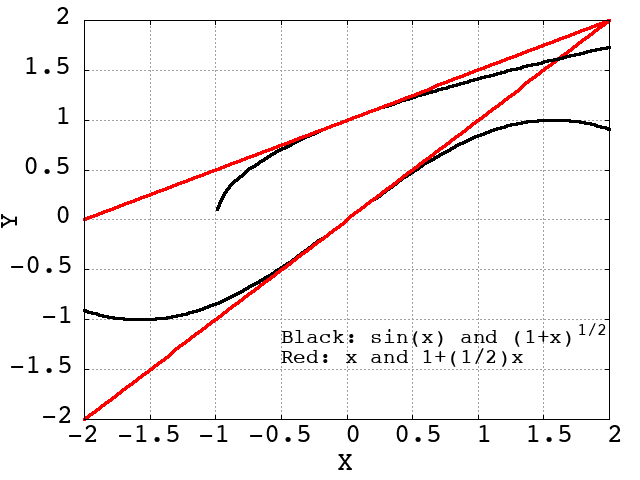
\includegraphics[width=0.7\textwidth]{figures/taylor_series.png}
\caption{\label{fig:approx} Certain functions may be approximated by simpler ones.  In this case, $\sin(x)$ is approximated by $x$ near $x=0$, and $(1+x)^{1/2}$ is approximated by $1+\frac{1}{2}x$ near $x=0$.}
\end{figure}
\end{frame}

\begin{frame}{Methods of approximation - Function approximation}
\small
\begin{minipage}[b]{0.45\linewidth}
The height in meters of a surfer above some average height as he bobs in the waves is described by $h(t) = sin(t)$.  What is his height at 1.0 second?  What is his height at -1.0 second?
\vspace{0.2cm}
\begin{itemize}
\item A: 1 meter, -1 meter
\item B: $\pi$ meters, -$\pi$ meters
\item C: -1 meter, 1 meter
\item D: -$\pi$ meters, $\pi$ meters
\end{itemize}
\end{minipage}
\hspace{0.5cm}
\begin{minipage}[b]{0.45\linewidth}
The value of an investment in dollars, $v$, versus time in years, $t$, follows the form $v(t) = P\exp(rt)$, where $P$ is the value at $t=0$, and $r=1/3$.  What is $v(1)$, the value after one year?
\vspace{0.6cm}
\begin{itemize}
\item A: $\approx 1/3 P$
\item B: $\approx 2/3 P$
\item C: $\approx 3/2 P$
\item D: $\approx 4/3 P$
\end{itemize}
\end{minipage}
\end{frame}

\begin{frame}{Methods of approximation - Units (Chapters 1.4-1.5)}
Physics requires \alert{units} to relate ideas to the real world, and \alert{unit analysis} is a powerful tool to eliminate incorrect results and to facilitate estimation.
\begin{enumerate}
\item SI units, and kilogram-meter-second unit set
\begin{itemize}
\item mass: \alert{kilogram} (gram = $10^{-3}$ kg, milligram = $10^{-6}$ kg)
\item length: \alert{meter} (millimeter = $10^{-3}$ m, kilometer = $10^{3}$ m)
\item time: \alert{second} (1 year $\approx \pi \times 10^{7}$ sec, 1 hour = 3600 sec)
\end{itemize}
\item Unit analysis
\begin{itemize}
\item If we are calculating a density, the units should work out to be kg/m$^3$
\item Identifying the fundamental unit in a complex calculation often simplifies it (when done properly, this reveals the beauty of physics)
\end{itemize}
\end{enumerate}
\end{frame}

\begin{frame}{Methods of approximation - Units (Chapters 1.4-1.5)}
\small
\begin{minipage}[b]{0.45\linewidth}
A millenium is 1000 years.  If a glacier retreats at a pace of 10 cm per year, what is this rate in meters per millenium?
\vspace{0.2cm}
\begin{itemize}
\item A: 0.1 meter per millenium
\item B: 1 meter per millenium
\item C: 10 meters per millenium
\item D: 100 meters per millenium
\end{itemize}
\end{minipage}
\hspace{0.5cm}
\begin{minipage}[b]{0.45\linewidth}
Ice has a density of 0.917 grams per centimeter cubed.  What is this density in kilograms per meter cubed?
\vspace{1.1cm}
\begin{itemize}
\item A: 91.7 kg/m$^3$
\item B: 917 kg/m$^3$
\item C: 9170 kg/m$^3$
\item D: 9.17 kg/m$^3$
\end{itemize}
\end{minipage}
\end{frame}

\begin{frame}{Methods of approximation - Units (Chapters 1.4-1.5)}
\centering
Sometimes, the beauty of physics arrises from choosing the right unit. \\
\vspace{1cm}
\small
\boxed{http://joshworth.com/dev/pixelspace/pixelspace\_solarsystem.html} \\
\vspace{1cm}
\normalsize
The Sun in this ruler is at 0 km, and Jupiter is at about 780,000,000 km (good luck finding it).  Clearly, the kilometer is the wrong unit to choose for interplanetary distances.  What if we defined a new unit, the \alert{astronomical unit}, as the distance between the Earth and the Sun?
\end{frame}

\begin{frame}{Methods of approximation - Units (Chapters 1.4-1.5)}
Planetary orbital radii in \alert{AU} (geometric means):
\begin{figure}
\begin{tabular}{| c | c |}
\hline
Mercury & 0.379 \\
Venus & 0.722 \\
Earth & 1.00 \\
Mars & 1.52 \\
Jupiter & 5.20 \\
Saturn & 9.54 \\
Uranus & 19.2 \\
Neptune & 30.1 \\
\hline
\end{tabular}
\caption{\label{tab:planets} Why such simple numbers?  There is a set of simple relationships between the \textit{orbital period} and the \textit{orbital radius} of planets called Kepler's Laws, which led to the discovery of \alert{Newton's Law of Gravity.}}
\end{figure}
\end{frame}

\section{Answers}

\begin{frame}{Answers}
\begin{itemize}
\item Mass of ants: 0.1 kg
\item Mass of baby whale: 5 tonnes
\item Length of flight is 10 hours
\item Number of birds is 10,000
\item Height of surfer is 1.0 meter, -1.0 meter
\item Value of investment is $4/3 P$
\item The glacier is retreating at 100 meters per millenium
\item Ice has a density of 917 kg/m$^3$
\end{itemize}
\end{frame}

\end{document}